% $Id$ %

The \setting{\label{ref:PlaybackSettings}Playback Settings} menu allows 
you to configure settings related to audio playback.

\section{Shuffle}
  Turning shuffle on will cause Rockbox to randomly re-order the
  playlist. Thus, to shuffle all of the audio files on the player, you first
  need to create a playlist containing all of them. For more information on
  creating playlists refer to \reference{ref:working_with_playlists}.\\
  Options: \setting{Yes}/\setting{No}.
  %
\section{Repeat}
  Configures settings related to repeating of directories or playlists.\\
  Options: \setting{Off} / \setting{All} / \setting{One} / \setting{Shuffle} /
  \setting{A-B}:
  \begin{description}
    %
  \item[Off.] The current playlist will not repeat when it is finished.
    \note{If you have the \setting{Auto-Change Directory} option set to
      \setting{Yes}, Rockbox will move on to the next directory on your
      hard drive. If the \setting{Auto-Change Directory} option is set to
      \setting{No}, playback will stop when the current directory or
      playlist is finished.}
    %
  \item[All.] The current playlist will repeat when it is finished.

    %
  \item[One. ]Repeat one track over and over.
    %
  \item[Shuffle.] When the current playlist has finished playing, it will
    be shuffled and then repeated.
    %
  \item[A-B.] Repeats between two user defined points within a track,
    typically used by musicians when attempting to learn a piece of music.
    This option is more complicated to use than the others as the \dap\
    must first be placed into A-B repeat mode and then the start and end
    points defined.\\

    \opt{RECORDER_PAD,IRIVER_H100_PAD,IRIVER_H300_PAD,IRIVER_H10_PAD,MROBE100_PAD%
        ,GIGABEAT_PAD,GIGABEAT_S_PAD,SANSA_E200_PAD,SANSA_C200_PAD}{%
        To set the Start Point (A) press \ActionWpsAbSetAPrevDir{}.
        Setting the End Point (B) is done accordingly using
        \ActionWpsAbSetBNextDir{}.  To reset the markers press \ActionWpsAbReset{}.
    }%
    \opt{ipod,IAUDIO_X5_PAD,ONDIO_PAD,PLAYER_PAD}{%
        To set the Start Point (A) press \ActionWpsBrowse{}. The following
        press of \ActionWpsBrowse{} will set the End Point (B), and a third
        successive \ActionWpsBrowse{} will reset the markers.
    }%
  \end{description}

\section{Play Selected First}
  This setting controls what happens when you
  select a file for playback while shuffle mode is on. If the
  \setting{Play Selected First} setting is \setting{Yes}, the file you
  selected will be played first. If this setting is \setting{No}, a random
  file in the directory will be played first.

\section{Fast-Forward/Rewind}
  These settings control the speed and acceleration during fast forward and rewind.
  The setting \setting{FF/RW Min Step} controls the initial speed and \setting{FF/RW Accel} controls the acceleration.

\opt{disk_storage}{
  \section{Anti-Skip Buffer}
    This setting controls how early Rockbox starts refilling the music buffer
    from the hard drive when playing. A longer Anti-Skip Buffer helps prevent
    skips in music playback if Rockbox has trouble reading from the disk.
    This can happen if the \dap{} is knocked, shaken or jogged heavily while
    Rockbox is trying to read the hard drive.

    \opt{masd,masf}{
      The anti-skip buffer can be set to a value between 0 and 7
      seconds.\\
    }

    \opt{swcodec}{
      The anti-skip buffer can be set to various values between
      5 seconds and 10 minutes.\\
    }

    \note{Having a large anti-skip buffer tends to use more power, and may
      reduce your battery life. It is recommended to always use the lowest
      possible setting that allows correct and continuous playback.}
}

\section{Fade on Stop/Pause}
  Enables and disables a fade effect when you
  pause or stop playing a song. If the Fade on Stop/Pause option is
  set to \setting{Yes}, your music will fade out when you stop or pause 
  playback, and fade in when you resume playback.
    
\section{Party Mode}
  Enables unstoppable music playback. When new songs are
  selected, they are queued at the end of the current dynamic playlist
  instead of being played immediately. Pausing and stopping playback is
  disabled as well as skipping songs and launching plugins.

\opt{swcodec}{
  \section{Crossfade}
    This setting enables a cross-fader. At the end of a song, the song will 
    fade out as the next song fades in, creating a smooth transition between 
    songs. The crossfade setting is particularly effective when the player is 
      set on shuffle.\\

    Options for crossfade settings are:
    \begin{description}
      \item[Enable Crossfade.] If set to \setting{Off}, crossfade is disabled.
	    If set to \setting{Auto Track Skip Only}, crossfade occurs for
        automatic skips, but not for manual skips.  The next setting,
        \setting{Manual Track Skip Only}, is the opposite: tracks will only
        crossfade when manually skipped.  If set to \setting{Shuffle}, crossfade
        is enabled for all track changes when the shuffle feature is set to
        \setting{Yes}, but disabled otherwise.  If set to
        \setting{Shuffle and Manual Track Skip} then crossfade will only be
        active when shuffle is set to \setting{Yes} and the track is then
        manually skipped.  If set to \setting{Always}, tracks will always
        crossfade into one another.
        %
      \item[Fade In Delay.] The ``fade in delay'' is the length of time between
        when the crossfade process begins and when the new track begins to fade
        in.
        %
      \item[Fade In Duration.] The length of time, in seconds, that it takes
        your music to fade in once the \setting{Fade In Delay} has ended.
        %
      \item[Fade Out Delay.] The ``fade out delay'' is the length of time
        between when the crossfade process begins and when the old track begins
        to fade out.
        %
      \item[Fade Out Duration.] The length of time, in seconds, that it takes
        your music to fade out once the \setting{Fade Out Delay} has ended.
        %
      \item[Fade Out Mode.] If set to \setting{Crossfade}, one song will fade
        out and the next song will simultaneously fade in. If set to 
        \setting{Mix}, the ending song will continue to play as normal until 
        its end, while the starting song will fade in from under it. 
        \setting{Mix} mode is not
        used for manual track skips, even if it is selected here.
      \end{description}
      
      \note{The rules above apply except in the instance where
          \setting{Fade Out Delay} plus \setting{Fade Out Duration} is less then
          \setting{Fade In Delay} (which would create a gap in the audio). In this case,
          the \setting{Fade In Delay} is reduced to eliminate the gap.\\}

          The graphic below illustrates how the different settings work in practice.

         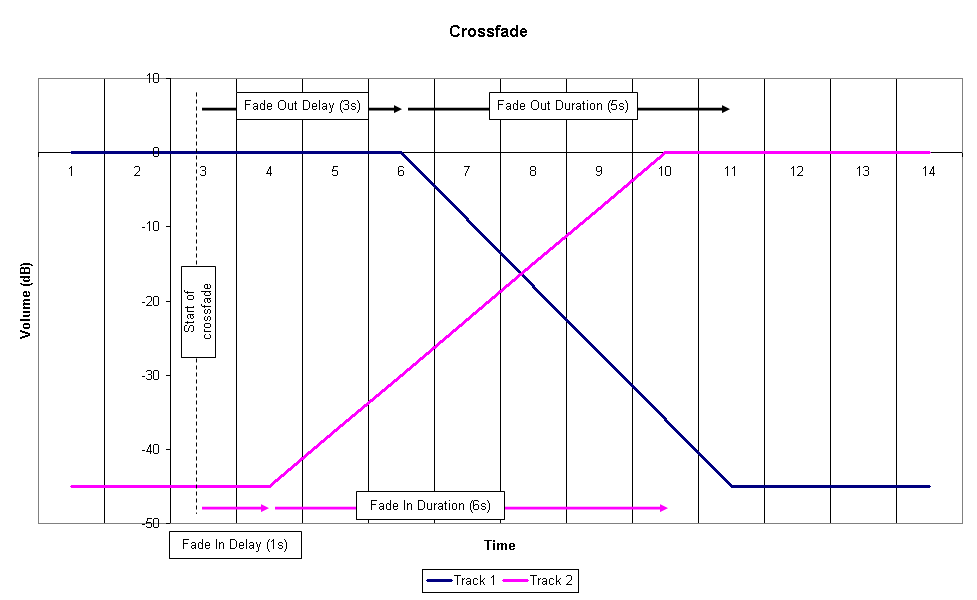
\includegraphics[width=14cm]{configure_rockbox/images/crossfade_graphic.png}
    
  \section{Replaygain}
    This allows you to control the replaygain function.
    The purpose of replaygain is to adjust the volume of the music played
    so that all songs (or albums, depending on your settings) have the
    same apparent volume. This prevents sudden changes in volume when
    changing between songs recorded at different volume levels.
    For replaygain to work, the songs must have been processed by a program
    that adds replaygain information to the ID3 tags (or Vorbis tags).\\

    \note{APEv2 tags are not currently supported.\\}
      
    Options for replaygain are:
    \begin{description}
      \item[Replaygain Type.] Choose the type of replaygain to apply:
        \begin{description}
        \item[Album Gain.] Maintain a constant volume level between
          albums, but keep any intentional volume variations between 
          songs in an album. (If album gain value is not available,
          uses track gain information).
          %
        \item[Track Gain.] Maintain a constant volume level between
          tracks. If track gain value is not available, no replaygain 
          is applied.
          %
        \item[Track Gain If Shuffling.] Maintains a constant volume
          between tracks if \setting{Shuffle} is set to \setting{Yes}.
          Reverts to album mode if \setting{Shuffle} is set to \setting{No}.
          %
        \item[Off.] Do not process replaygain information, i.e. turn off
          the replaygain function.
        \end{description}
        %
      \item[Prevent Clipping.] Avoid clipping of a song's waveform.
        If a song would clip during playback, the volume is lowered for 
        that song. Replaygain information is needed for this to work.
        %
      \item[Pre-amp.] This allows you to adjust the volume when replaygain
        is applied. Replaygain often lowers the volume, sometimes quite
        much, so here you can compensate for that. Please note that a
        (large) positive pre-amp setting can cause clipping, unless
        prevent clipping is enabled.  The pre-amp can be set to any
        decibel (dB) value between -12dB and +12dB, in increments of 0.1{}dB.
      \end{description}

  \section{Track Skip Beep}
    Controls the volume of the beep that is heard when
    skipping forward or backward between tracks. The beep is disabled when
    set to \setting{Off}.
}%\opt{swcodec}

\opt{spdif_power}{
  \section{Optical Output}
    Enables or disables the optical S/PDIF output to 
    allow a digital connection to a suitable external decoder.  To enable
    optical output, set to \setting{Yes}
}

\section{Auto-Change Directory}
  Control what Rockbox does when it reaches the end
  of a directory. If \setting{Auto-Change Directory} is set to \setting{Yes},
  Rockbox will continue to the next directory. If
  \setting{Auto-Change Directory} is set to \setting{No}, playback will stop at
  the end of the current playlist.  Using the \setting{Random} feature requires
  you to first generate a folder list via the Random Folder Advance Configuration
  plugin (see \reference{ref:random_folder_advance_config}).\\

  \note{You must have the \setting{Repeat} option set to \setting{No} for
    \setting{Auto-Change Directory} to function properly.\\}

  \note{This feature only works when songs have been played from the file
    browser.  Using it with the database may cause unexpected behaviour.}

  %
\opt{headphone_detection}{
\section{Pause on Headphone Unplug}
  Enables and disables automatic pausing of 
  playback when the headphones are disconnected from the \daps{} headphone 
  socket.
  %
  \begin{description}
  \item[Pause on Headphone Unplug.] Options for automatic pause:
    \begin{description}
    \item[Off.] Disables automatic pause.
      %
    \item[Pause.] Pauses the \dap{} when the headphones are removed.
      %
    \item[Pause and Resume.] Pauses when the headphones are removed, and 
      resumes playback when they are reconnected.
  \end{description}
  \item[Duration to Rewind.] Number of seconds (between 0 and 15) to rewind 
    playback when the headphones are removed.
    %
  \item[Disable Auto-Resume If Phones Not Present.] This option will disable 
    the automatic resumption of playback at startup if the headphones are not 
    connected to the \dap{}.
    \note{This requires \setting{Resume on Startup} to be enabled.}
  \end{description}

}%

\section{Last.fm Log}\index{Last.fm Log}\index{Audioscrobbler|see{Last.fm Log}}
  Enables logging of your played tracks for submittal to 
  \url{http://www.last.fm}. This service was formely known as 
  \emph{Audioscrobbler}. When you enable this option, you'll have to reboot to
  start the logging. The log-file is called 
  \opt{rtc}{\fname{.scrobbler.log},}%
  \nopt{rtc}{\fname{.scrobbler-timeless.log},}%
  and is to be found in the root directory of your \dap{}.\\

  \note{See \wikilink{LastFMLog} for a further description, and for tools you 
    can use to submit your Last.fm log.}

\section{Cuesheet Support}\index{Cuesheet Support}
  Enables reading of cuesheet files for played tracks. If a cuesheet is found
  for a track, track markers are displayed on the progressbar and it is
  possible to skip between the tracks within the cuesheet. Also the information
  found in the cuesheet file will replace the information from the ID3 tags.
  When you enable this option, you'll have to reboot for it to come into
  effect.
  
\section{Skip Length}\index{Skip Length}
  Designed to speed up navigation when listening to long audio tracks,
  \setting{Skip Length} changes the behaviour of
  the \ActionWpsSkipPrev{} and \ActionWpsSkipNext{} buttons so that they skip
  by a given time instead of skipping to a new track.
  The \setting{Skip to Outro} option changes the behaviour so that the buttons
  skip to just before the end of the track, so that the last few seconds are
  played before the next track.

\section{Prevent Track Skipping}\index{Prevent Track Skipping}
  If this option is enabled, the ability to manually skip tracks is disabled
  in order to avoid accidental track skips. It does not prevent changing tracks
  if a track ends, which can be achieved by combining this option with
  \setting{Repeat} set to \setting{One}

